\documentclass[a4wide,10pt]{scrartcl}
\usepackage[utf8]{inputenc}
\usepackage{amsmath,amssymb}
\usepackage{graphicx}
\usepackage{caption}
\usepackage{subcaption}
\usepackage{listings}

\newcommand{\Dt}{\Delta t}

% Title Page
\title{Futurization of ODE integration}
\author{}


\begin{document}
\maketitle

Solving initial value problems (IVP) of ordinary differential equations (ODE) is an every-day problem for scientists an engineers in all subjects.
In the following we will show how typical numerical algorithms for finding approximate solutions of such IVP can be parallelized using a dataflow approach.
An IVP of an ODE is defined as:
\begin{equation}
 \dot{\vec x}(t) = \vec f(\vec x(t), t), \qquad \vec x(t=0) = \vec x_0,
\end{equation}
where $\vec x(t) \in \mathbb{R}^N$ is the trajectory in the $N$-dimensional phase space.
To find a numerical solution of this problem one introduces a time discretization with some step size $\Dt$.
So the numerical solution consists of a sequence of $N$-dimensional points $\vec x_0$, $\vec x_1$, $\vec x_2,\dots$, with $\vec x_n \approx x(n\cdot \Dt)$.
The most important class of schemes are the Runge-Kutta methods, which are explicit one-step methods that use only the previous point $x_n$ to compute the next iterate $x_{n+1}$.
The generic explicit Runge-Kutta scheme with $s$ stages writes as:
\begin{equation} \label{eqn:rk}
 \begin{aligned}
    \vec x_{n+1} &= \vec x_n + \Dt \sum_{k=1}^{s} b_k \vec y_k \\
    \text{where}\quad \vec y_k &= f( \vec x_n + \Dt \sum_{m=1}^k a_{k,m} \vec y_m , t_n+c_k\Dt).
   \end{aligned}
\end{equation}
The parameter sets $a_{k,m}$, $b_k$ and $c_k$ have to be chosen such that the result $x_{n+1}$ is indeed an approximation of some order $p$.
We note that for simplicity we here restrict the study to methods with constant step-size~$\Dt$, but the method below can also be applied to embedded Runge-Kutta schemes required for step size control.
To obtain an approximation of a whole trajectory from $t=0\dots t_\text{end}$ one applies the above one-step algorithm subsequently to obtain a descretized approximate trajectory $\vec x_0,\vec x_1,\vec x_2,\dots,\vec x_T$ with $T=t_\text{end}/\Dt$.

Looking at~\eqref{eqn:rk} one see that the computation of a numerical trajectory consists of two tasks: (i) evaluation the rhs of the ODE $\vec f(\vec x,t)$ and (ii) compute the sum of vector-scalar products $\sum b_k \vec y_k$.
To parallelize these computations one divides the $N$-dimensional vector $\vec x$ into $M$ sub regions $\vec x^{m}\in \mathbb{R}^{N/M}$, with $m=0\dots M-1$, or $\vec y^{m}$ respectively, which are then distributed across cores/processors/machines and are processed in parallel.
While for the vector addition the computations of the sub regions $\vec y^m$ are completely independent from each other, for the rhs $\vec f(\vec x , t)$ this not the case.
The dependency between the regions is given by the specific problem one is confronted with.
For example, for a system with all-to-all coupling (e.g.\ $N$-body gravitation system), the calculation of one part $\vec y^m$ requires the full state $\vec x^{0}\dots \vec x^{M-1}$.
For the trivial case of an uncoupled system the calculation of $\vec y^m$ only requires the single component $\vec x^m$.
Many systems, however, are somewhere in between these two extreme cases.
Imagine, for example, a problem with nearest neighbor coupling, a very common case in lattice dynamics simulations, then the computation of $\vec y^m$ requires the neighboring components as well: $\vec x^{m-1}$, $\vec x^{m}$ and $\vec x^{m+1}$.
With conventional methods, like OpenMP or MPI, it is not possible, or at least highly cumbersome, to incorporate the dependencies into the parallelized code.
Therefore, a global synchronization is enforced after every rhs evaluation and vector addition step, as shown in Figure~\ref{fig:glob_sync}.

Here, we present a new way of parallelizing the algorithm based on dataflow semantics, that will automatically ensure the correct dependencies between the sub-regions of $\vec x^m$.
A natural way of representing the sub-regions $\vec x^m$ in a C++ program is a vector of vectors \lstinline+vector< vector< double > > x+, where \lstinline+x[m]+ represents the $N/M$ dimensional sub-regions $\vec x^m$.
For the futurization of the algorithm one first replaces the plain data types by \lstinline+future+ objects holding this data.
I.e.\ the representation of the regions becomes \lstinline+vector< future< vector< double > > >+, where the future object gets ready as soon as the computation of its data is finished.
Having defined this data structure, it is now very simple to implement a vector-vector addition ready for parallel execution.
Our implementation is based on the \lstinline+hpx::lcos::local::dataflow+ function, that applies a functor to a number of future objects.
Exemplarily, we show the code that computes the sum of two vectors $\vec z = \alpha_1 \vec x_1 + \alpha_2 \vec x_2$ separately for each sub region so that the individual tasks can be distributed on the available cores by the HPX scheduler.
\begin{lstlisting}
typedef vector< double > sub_state;
typedef vector< future< sub_state > > state;

struct scale_sum2
{
  const double a1 , a2;
  vadd3( double alpha1 , double alpha2 )
    : a1( alpha1 ) , a2( alpha2 ) { }
    
  state operator()( sub_state x1 , sub_state x2 , sub_state x3 )
  {
    for( size_t n=0 ; n<x1.size() ; n++ )
    {
      x1[n] = a1*x2[n]+a2*x3[n];
    }
    return x1;
  }
};

template< typename Operation >
void vector_apply2( state x1 , state x2 , state x3 , Operation op )
{
  for( size_t m=0 ; m<x1.size() ; m++ )
  {
    x1[m] = dataflow( hpx::launch::async , op , x1[m] , x2[m] , x3[m] );
  }
}
...
//calculate z = 0.5*x1 + 0.25*x2
vector_apply( z , x1 , x2 , scale_sum( 0.5 , 0.25 ) );
\end{lstlisting}
The \lstinline+dataflow+ function schedules the execution of the vector operation on the sub-region as soon as all required data is available from the previous operation.
Secondly, one has to implement the rhs of the ODE.
Here, we will chose an autonomous system with nearest neighbor couplings as an example, but the generalization to other dependencies is rather straight forward.
The rhs of an ODE with nearest neighbor coupling in the most general form writes as:
\begin{equation}
 \dot{\vec x} = \vec f(\vec x):\, x_n = g_n(q_n) + c_{n,l}(q_{n},q_{n-1}) + c_{n,r}(q_{n},q_{n+1}).
\end{equation} 
The function $g_n$ defines the local term at site $n$, while the functions $c_{n,1/2}$ represent the couplings to the left and right.
For simplicity, we will assume that the rhs functions are identical for all lattice sites, and also the left and right coupling is identical, hence: $g_n \equiv g$ and $c_{n,l} \equiv c_{n,r} \equiv c$.
Also, we will employ Diriclet boundary conditions employing that $x[-1] = x[N] = 0$.
Then, the futurized algorithm to compute this function reads:
\begin{lstlisting}
struct rhs_operation
{
  sub_state operator()( sub_state dxdt , sub_state x , double x_l , double x_r )
  {
    const size_t N = x.size();
    dxdt[0] = g_func( x[0] ) + c_func( x[0] , x_l ) 
			     + c_func( x[0] , x[1] );
    for( size_t n=1 ; n<N-1 ; ++n )
    {
      dxdt[n] = g_func( x[n] ) + c_func( x[n] , x[n-1] ) 
			       + c_func( x[n] , x[n+1] );
    }
    dxdt[N-1] = g_func( x[N-1] ) + c_func( x[N-1] , x[N-2] ) 
				 + c_func( x[N-1] , x_r );
    return dxdt;
  }
};

void rhs( state x , state dxdt , double t )
{
  const size_t M = x.size();
  // boundary condition on the left
  dxdt[0] = dataflow( rhs_operation() , x[0] , dxdt[0] , 
      make_ready_future( 0.0 ) ,
      dataflow( []( sub_state x ){ return x[0]; } , x[1] ) );
  for( size_t m=1 ; m<x.size()-1 ; x++ )
  {
    dxdt[m] = dataflow( rhs_operation() , x[m] , dxdt[m] , 
      dataflow( []( sub_state x ){ return x[x.size()-1]; } , x[m-1] ),
      dataflow( []( sub_state x ){ return x[0]; } , x[m+1] ) );
  }
  // boundary condition on the right
  dxdt[M-1] = dataflow( rhs_operation() , x[M-1] , dxdt[M-1] , 
      dataflow( []( sub_state x ){ return x[x.size()-1]; } , x[M-2] ),
      make_ready_future( 0.0 ) );
}
\end{lstlisting}
Note, how in the function \lstinline+rhs+ dataflows are used to extract the first/last value of the neighboring regions and pass them into the next dataflow.
That implies that effectively the dataflow for calculating the rhs for the $m$-th sub-region gets input from the regions $m-1$, $m$ and $m+1$.
This is exactly the constitution of the dependencies of the nearest neighbor coupling.
With this technique, the computation of the rhs function for region $m$ starts as soon as all the required data is available, even if some other sub-regions are not yet computed.

In contrast, an OpenMP implementation of the rhs function could look like:
\begin{lstlisting}
void rhs( state x , state dxdt , double t )
{
  const size_t M = x.size();
  const size_t L = x[0].size();
  rhs_operation op;
#pragma omp parallel for schedule(static)
  for( size_t m=0 ; m<M ; ++m )
  {
    if( m==0 )
      dxdt[0] = op( x[0] , 0.0 , dxdt[1][0] );
    elseif( m<M-1 )
      dxdt[m] = op( x[m] , dxdt[m-1][L-1] , dxdt[m+1][0] );
    else
      dxdt[M-1] = op( x[M-1] , dxdt[M-2][L-1] , 0.0 );
  }
}
\end{lstlisting}
Note that here, the parallel code is only entered when the full state $\vec x$ is calculated completely.
Additionally, at the end of the parallel OpenMP region a global synchronization takes place.
The difference in the execution flow of these two methods is visualized in Figure~\ref{??}.

It is clear that for the case of identical computation for all sub-regions ($g_n$ and $c_n$ independent of $n$) and in a homogeneous multi-core environment, the punishment of a global synchronization at each step is not expected to be of significant impact.
However, we still compare the new futurization approach based on HPX with a standard OpenMP implementation for exactly such a case and we will find that the HPX code is competitive even in this setting highly favorable for OpenMP, as shown in Figure~\ref{fig:marvin_scaling}.

As example system for our performance comparison we choose a Hamiltonian system of nonlinearly coupled anharmonic oscillators.
The equations of motions for a one-dimensional chain of these oscillators is:
\begin{equation}
 \dot p_n = -|q_n|^\kappa - |q_n-q_{n-1}|^\lambda - |q_n-q_{n+1}|^\lambda.
\end{equation} 
Hence, the functions from above are set to $g(x) = x^\kappa$ and $c(x,y)=(x-y)^\lambda$.
This model with integer powers $\kappa$ and $\lambda$ has been studied extensively by theoretical physicists in the context of Hamiltonian Chaos and Chaotic Diffusion~\cite{blabla}.
Here, we will use non-integer powers $\kappa=2.5$ and $\lambda=3.5$, which makes the system even more computationally demanding.

\begin{figure}
 \begin{subfigure}[b]{0.49\textwidth}
  \centering
  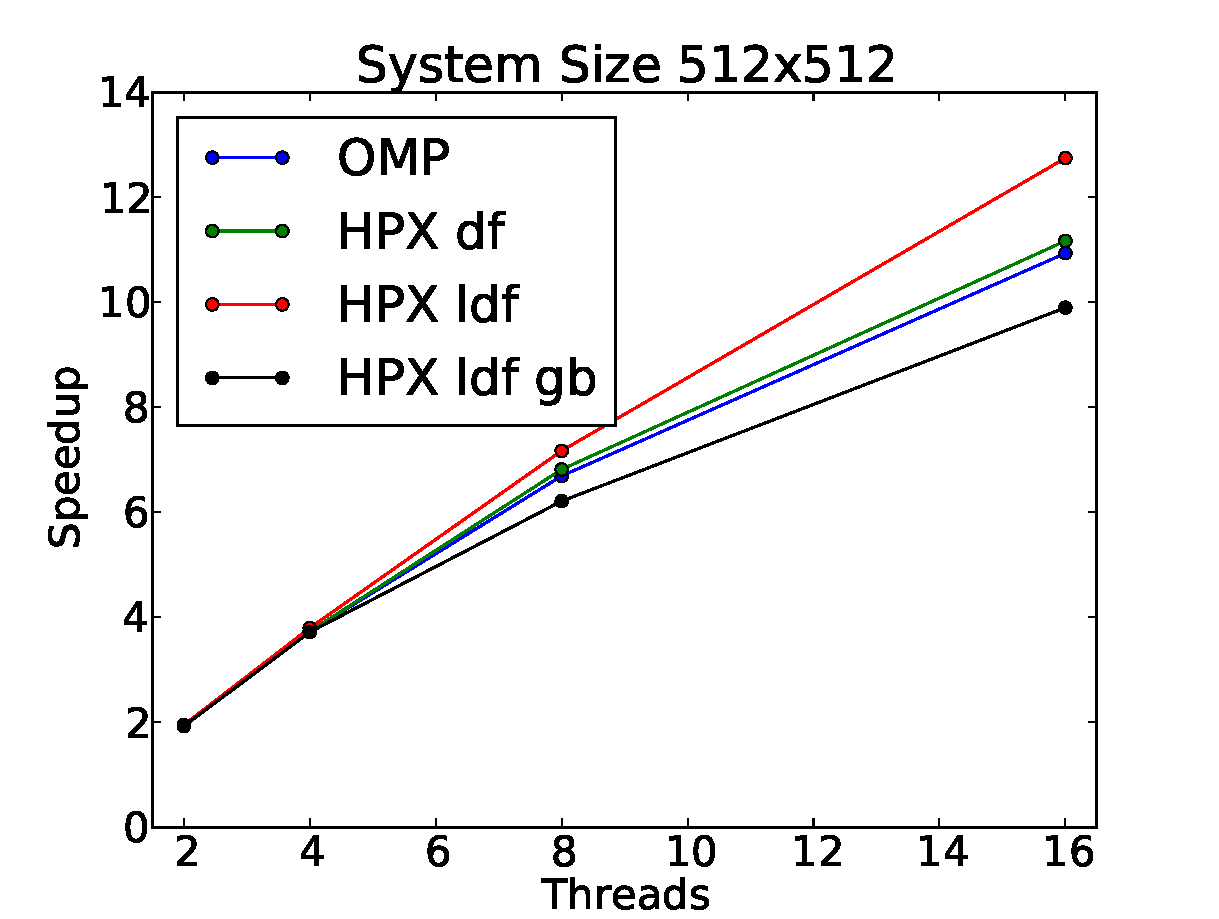
\includegraphics[width=\textwidth]{../plot/marvin_scaling_512.pdf}\hfill
  \caption{Performance with 512x512 lattice sites.} 
  \label{fig:scaling_marvin_512}
 \end{subfigure}
 \begin{subfigure}[b]{0.49\textwidth}
  \centering
  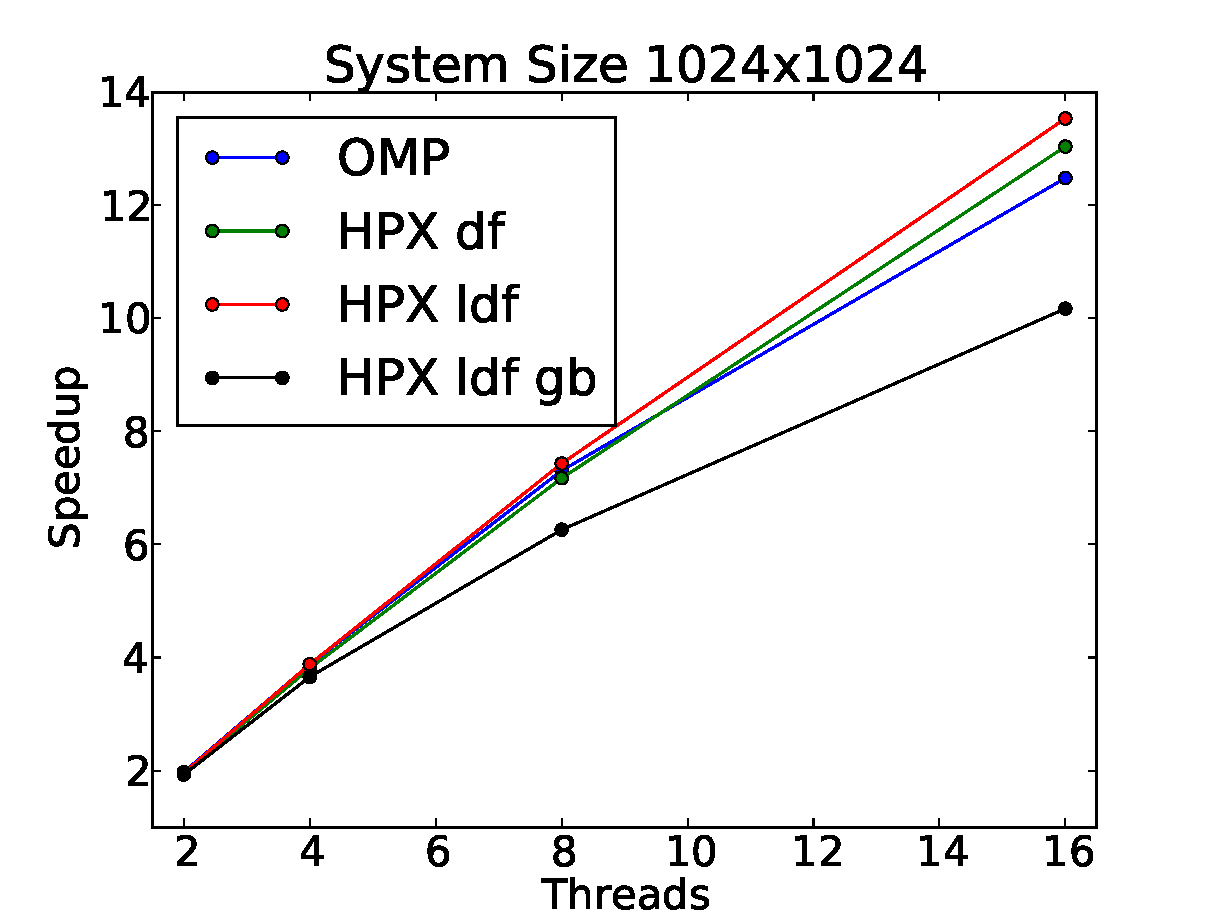
\includegraphics[width=\textwidth]{../plot/marvin_scaling_1024.pdf}\hfill
  \caption{Performance with 1024x1024 lattice sites.} 
  \label{fig:scaling_marvin_1024}
 \end{subfigure}
 \caption{Strong scaling for a system of size 512x512 (a) and 1024x1024(b) on a 2xXeonE5-2450 with 16 Cores (no Hyperthreading). The black curve (``HPX ldf gb'') represents the performance of a simulation using HPX local dataflows with additional global barriers.}
 \label{fig:marvin_scaling}
\end{figure}

\end{document}
